\section{Results}

\subsection{Grid}

We evaluated the performance of the Grid method with a 50x50 grid. Figure~\ref{fig:grid} shows simulation snapshots of the grid simulation.

\begin{figure*}[h]
    \centering
    \begin{subfigure}[b]{0.2\textwidth}
        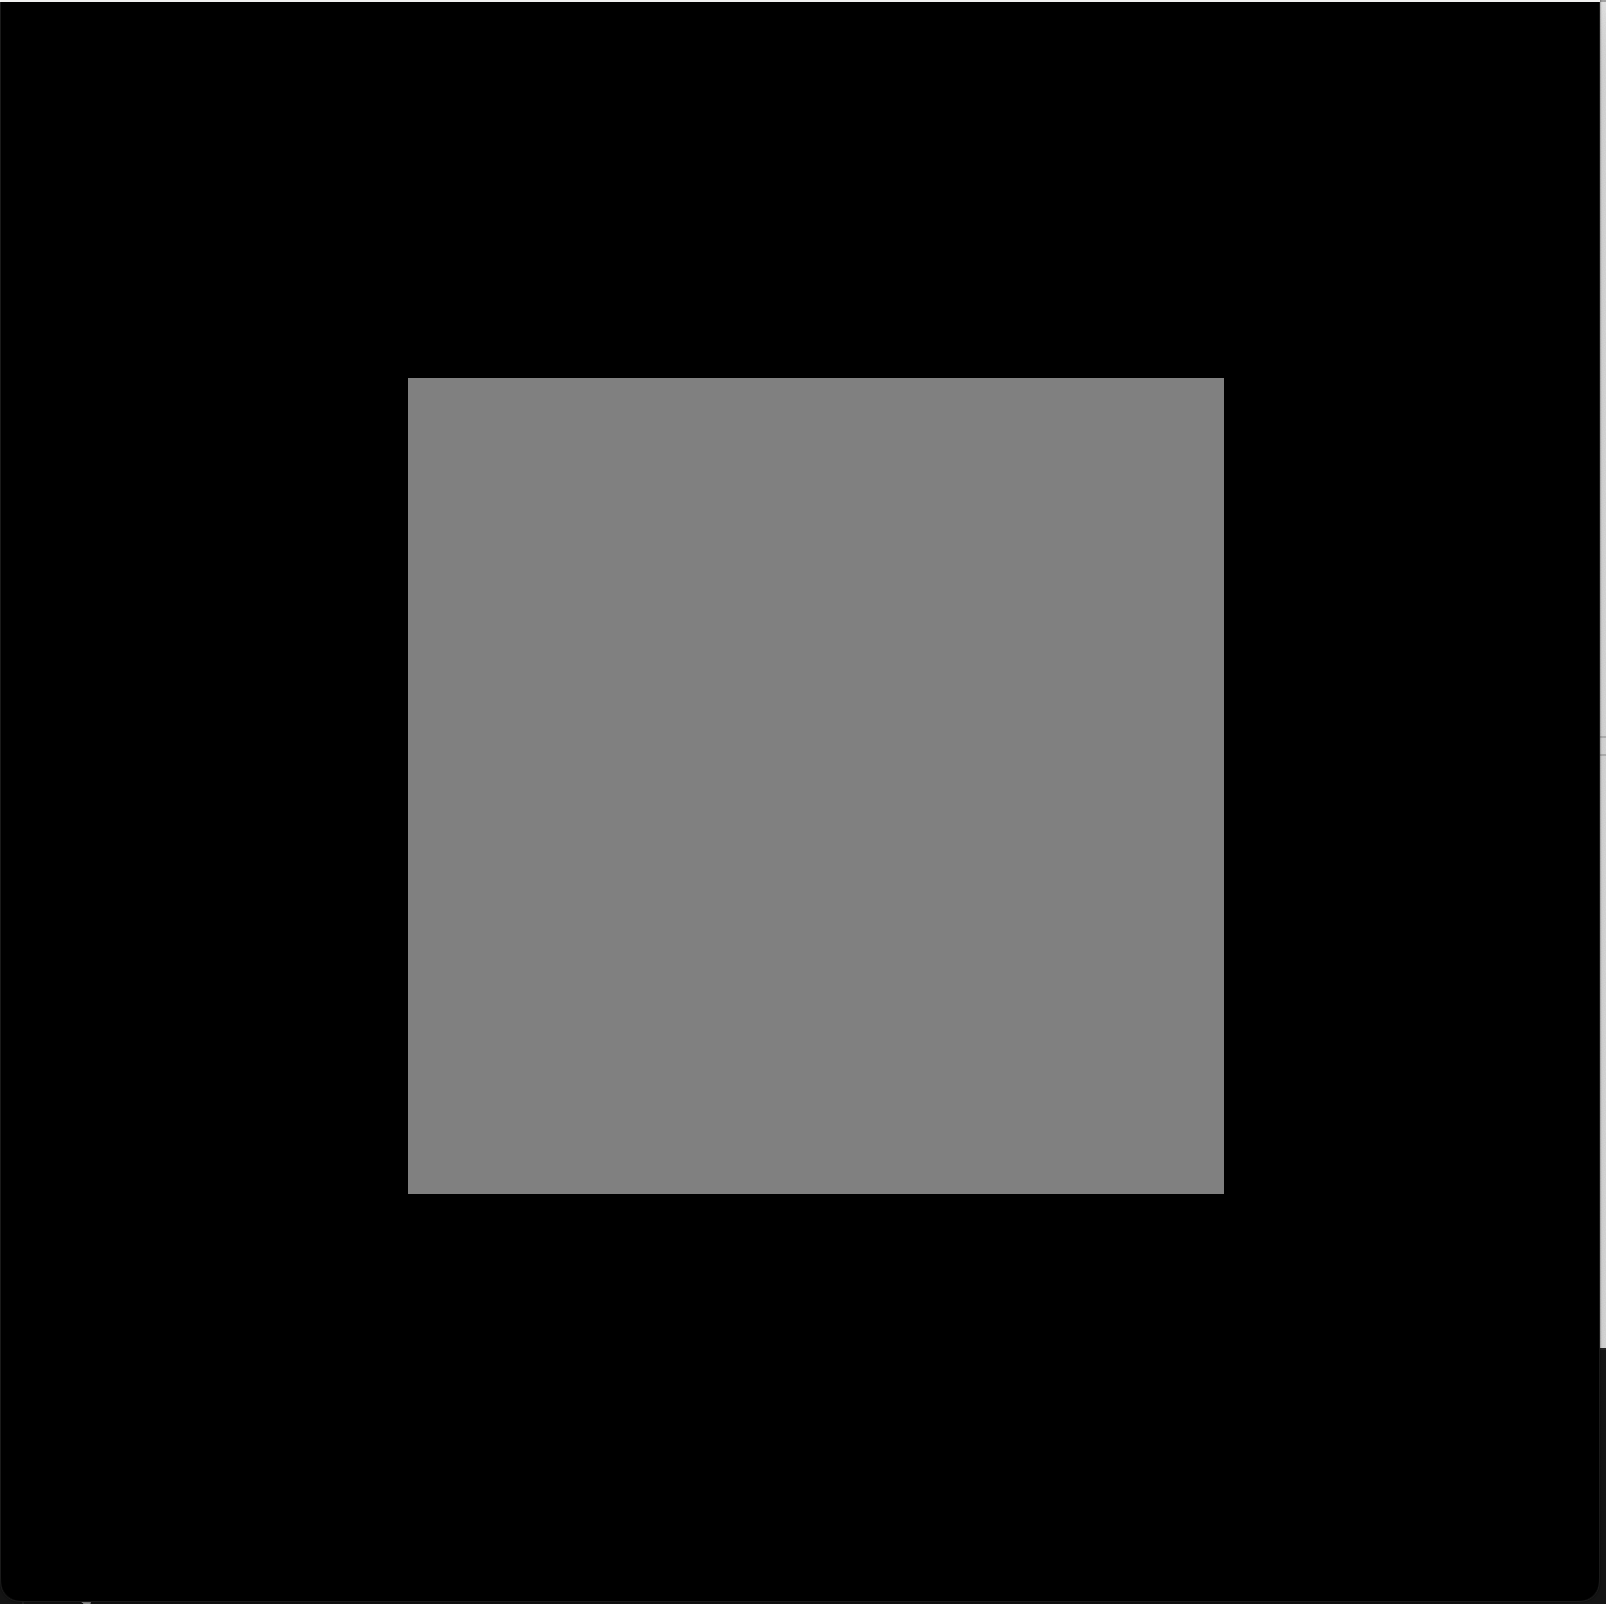
\includegraphics[width=\textwidth]{figures/grid50_init.png}
        \caption{initialization}
    \end{subfigure}
    \hspace{1em}
    \begin{subfigure}[b]{0.2\textwidth}
        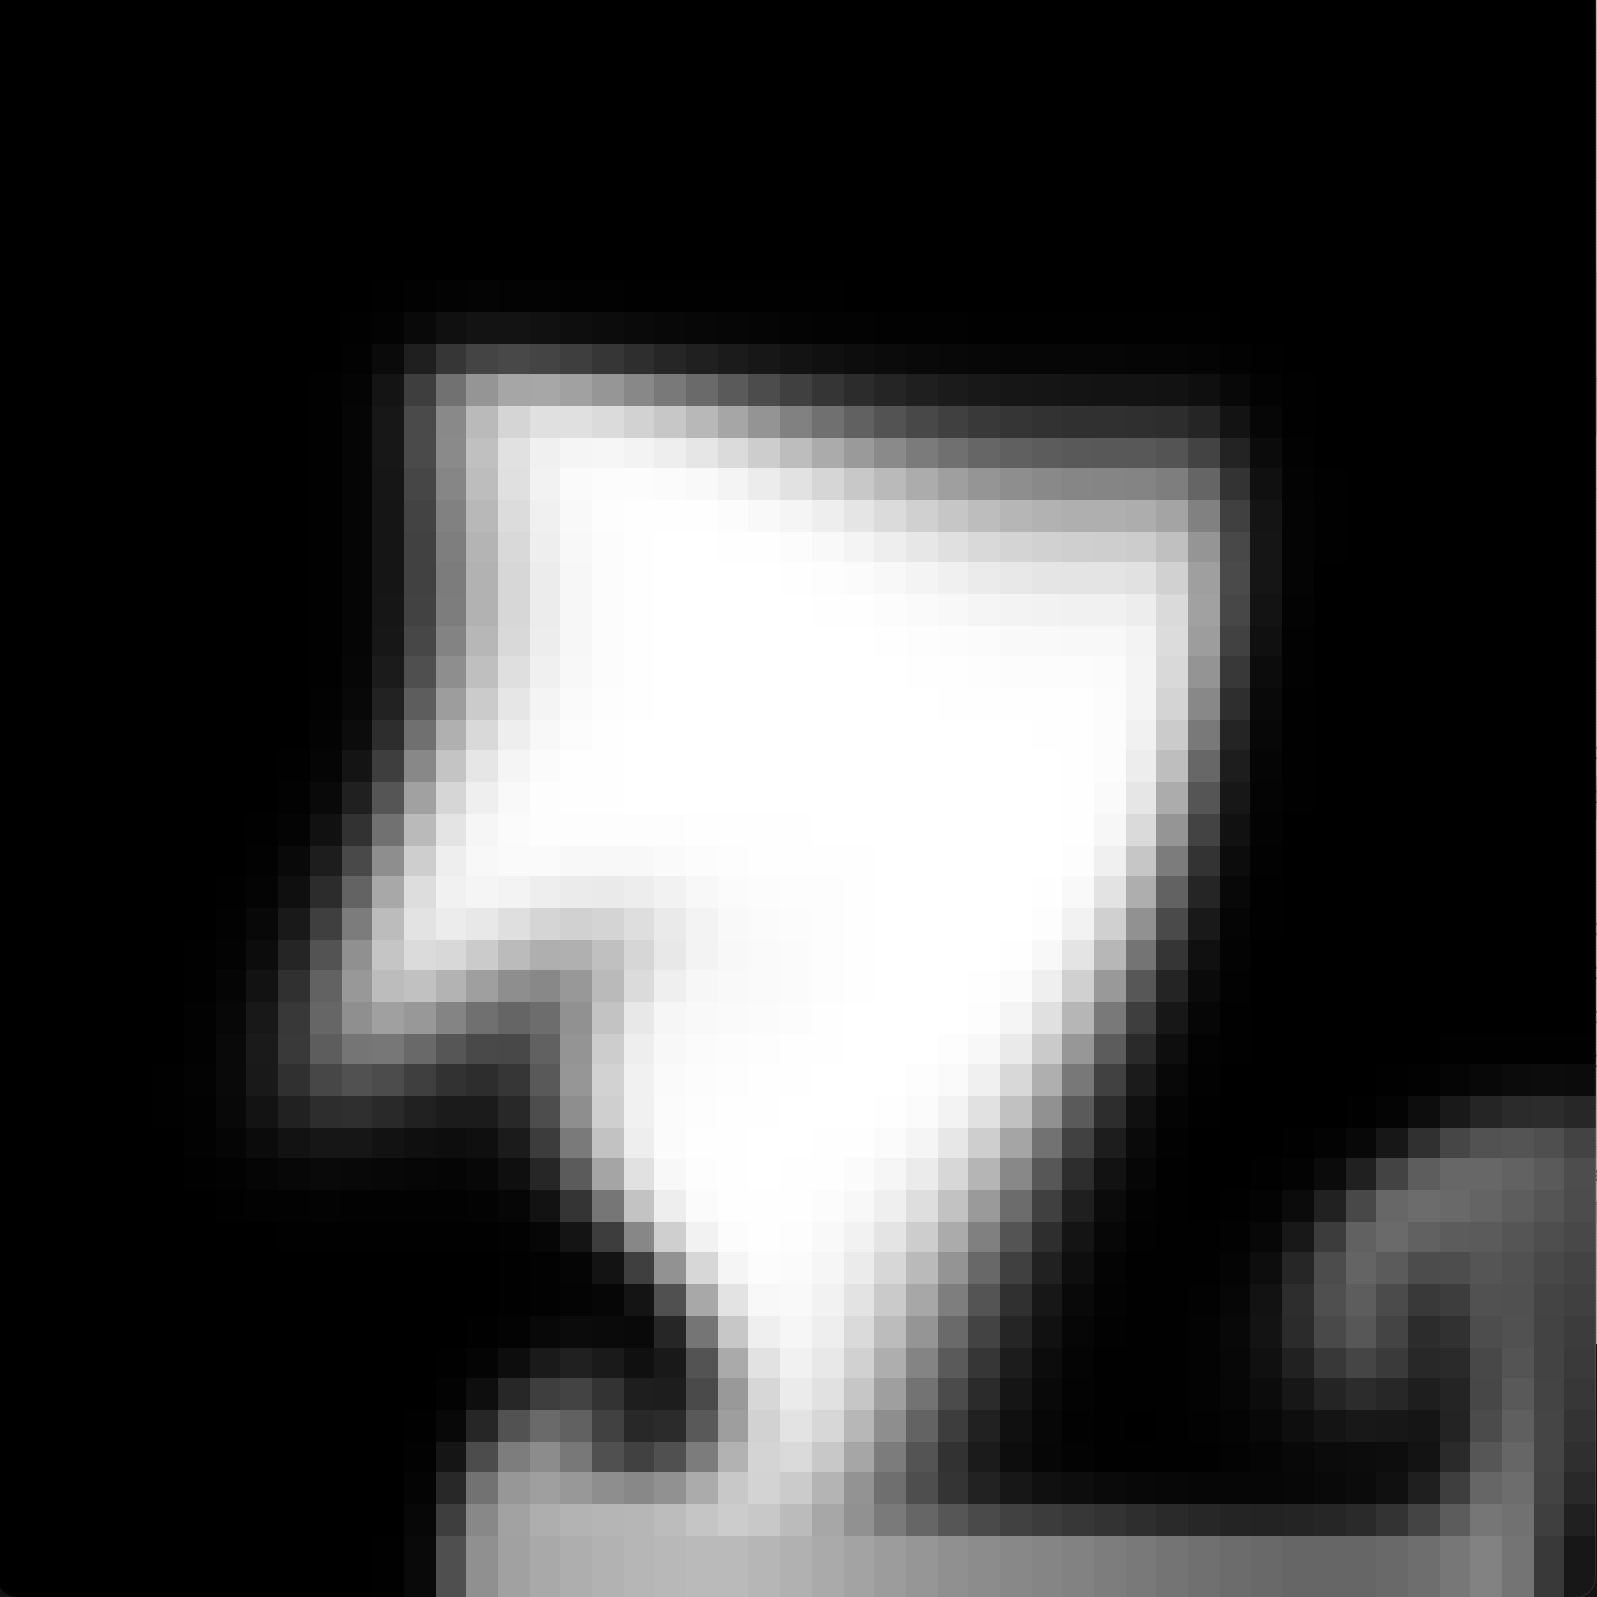
\includegraphics[width=\textwidth]{figures/grid50_1.png}
        \caption{first stage}
    \end{subfigure}
    \hspace{1em}
    \begin{subfigure}[b]{0.2\textwidth}
        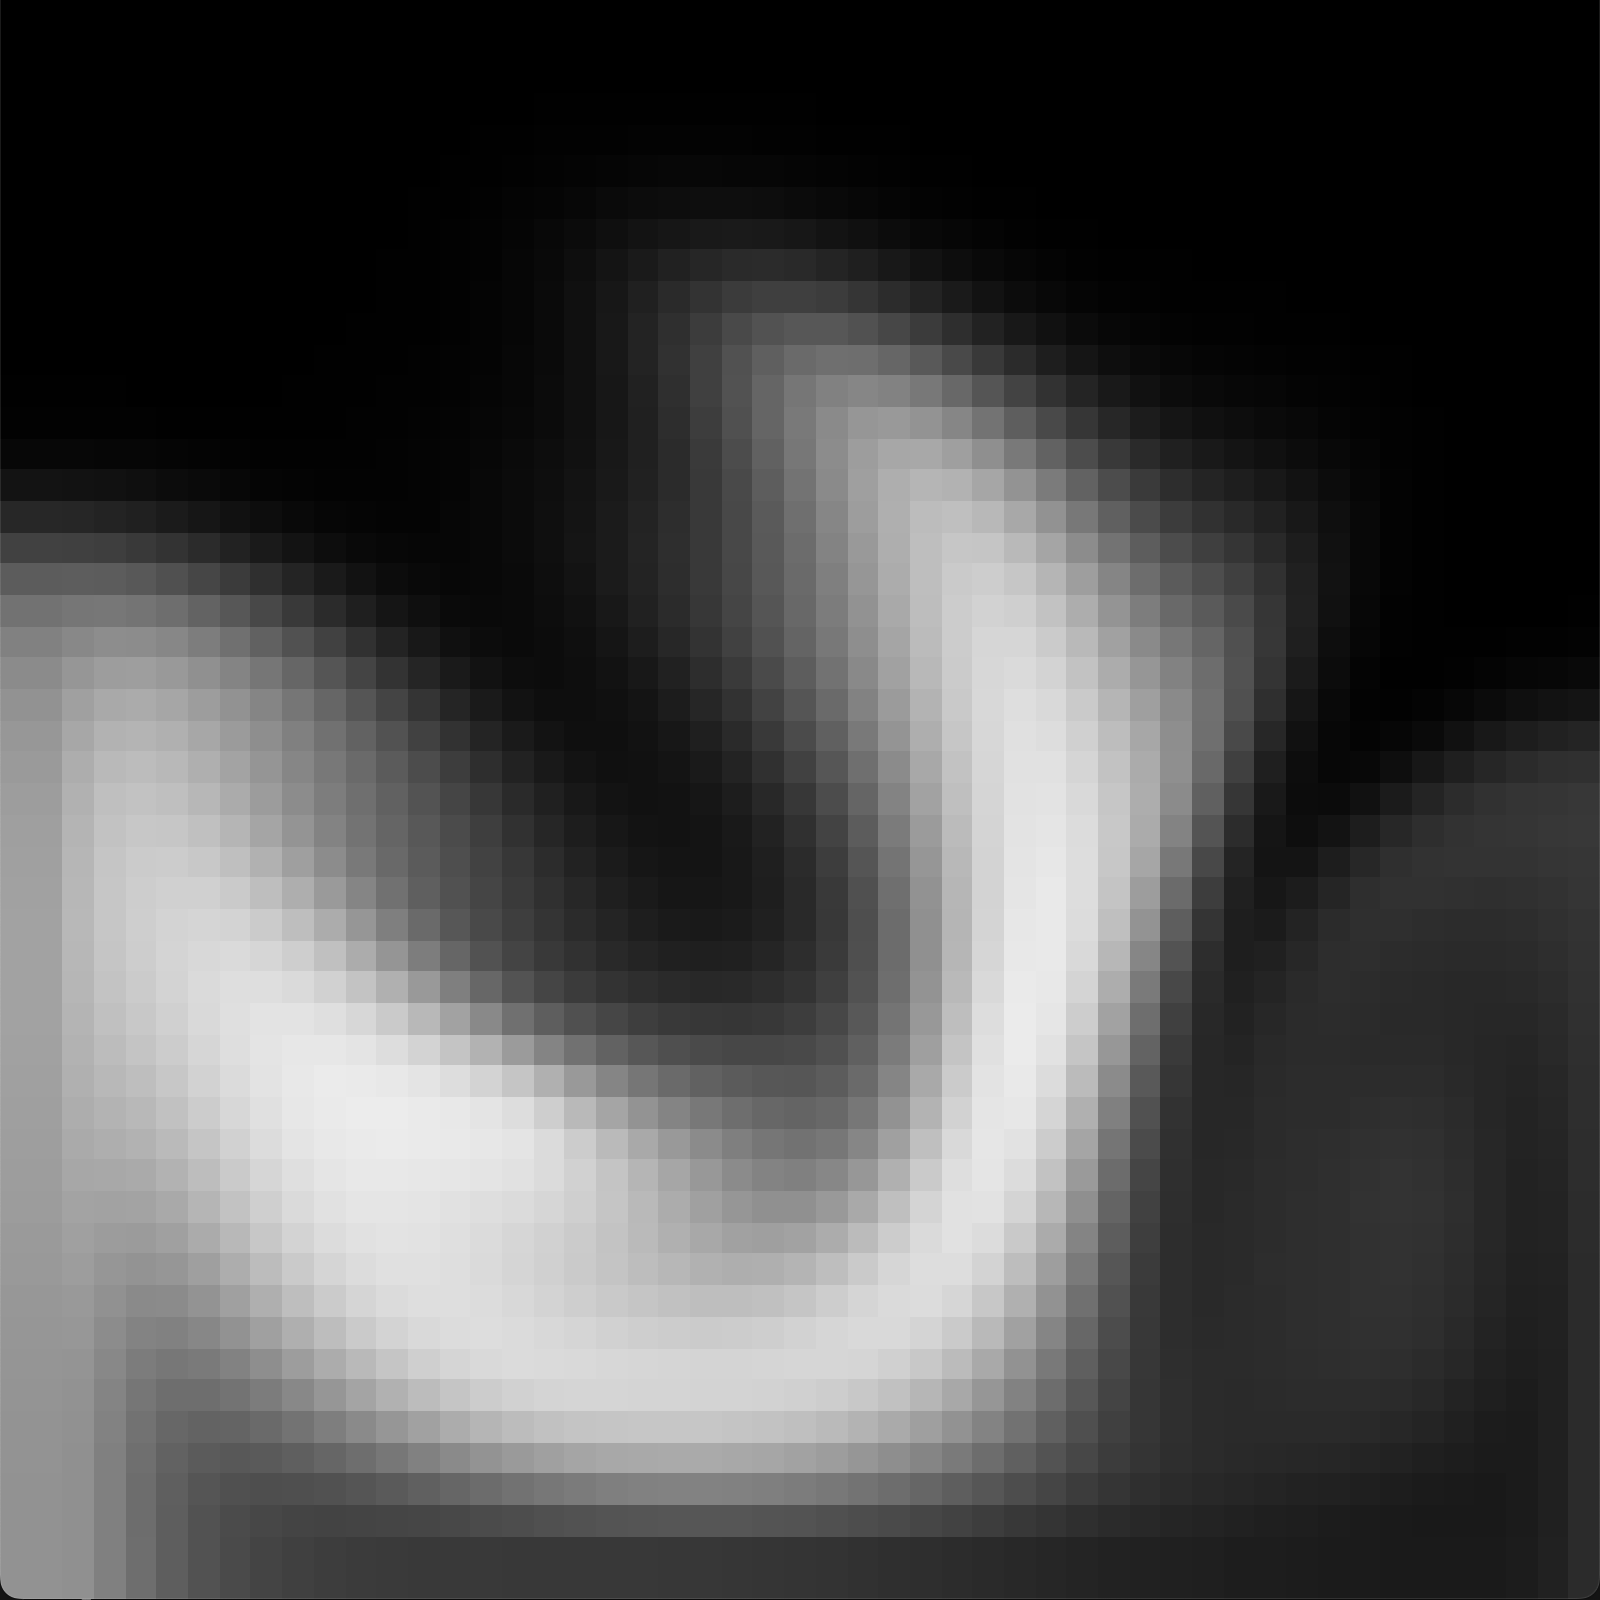
\includegraphics[width=\textwidth]{figures/grid50_2.png}
        \caption{second stage}
    \end{subfigure}
    \hspace{1em}
    \begin{subfigure}[b]{0.2\textwidth}
        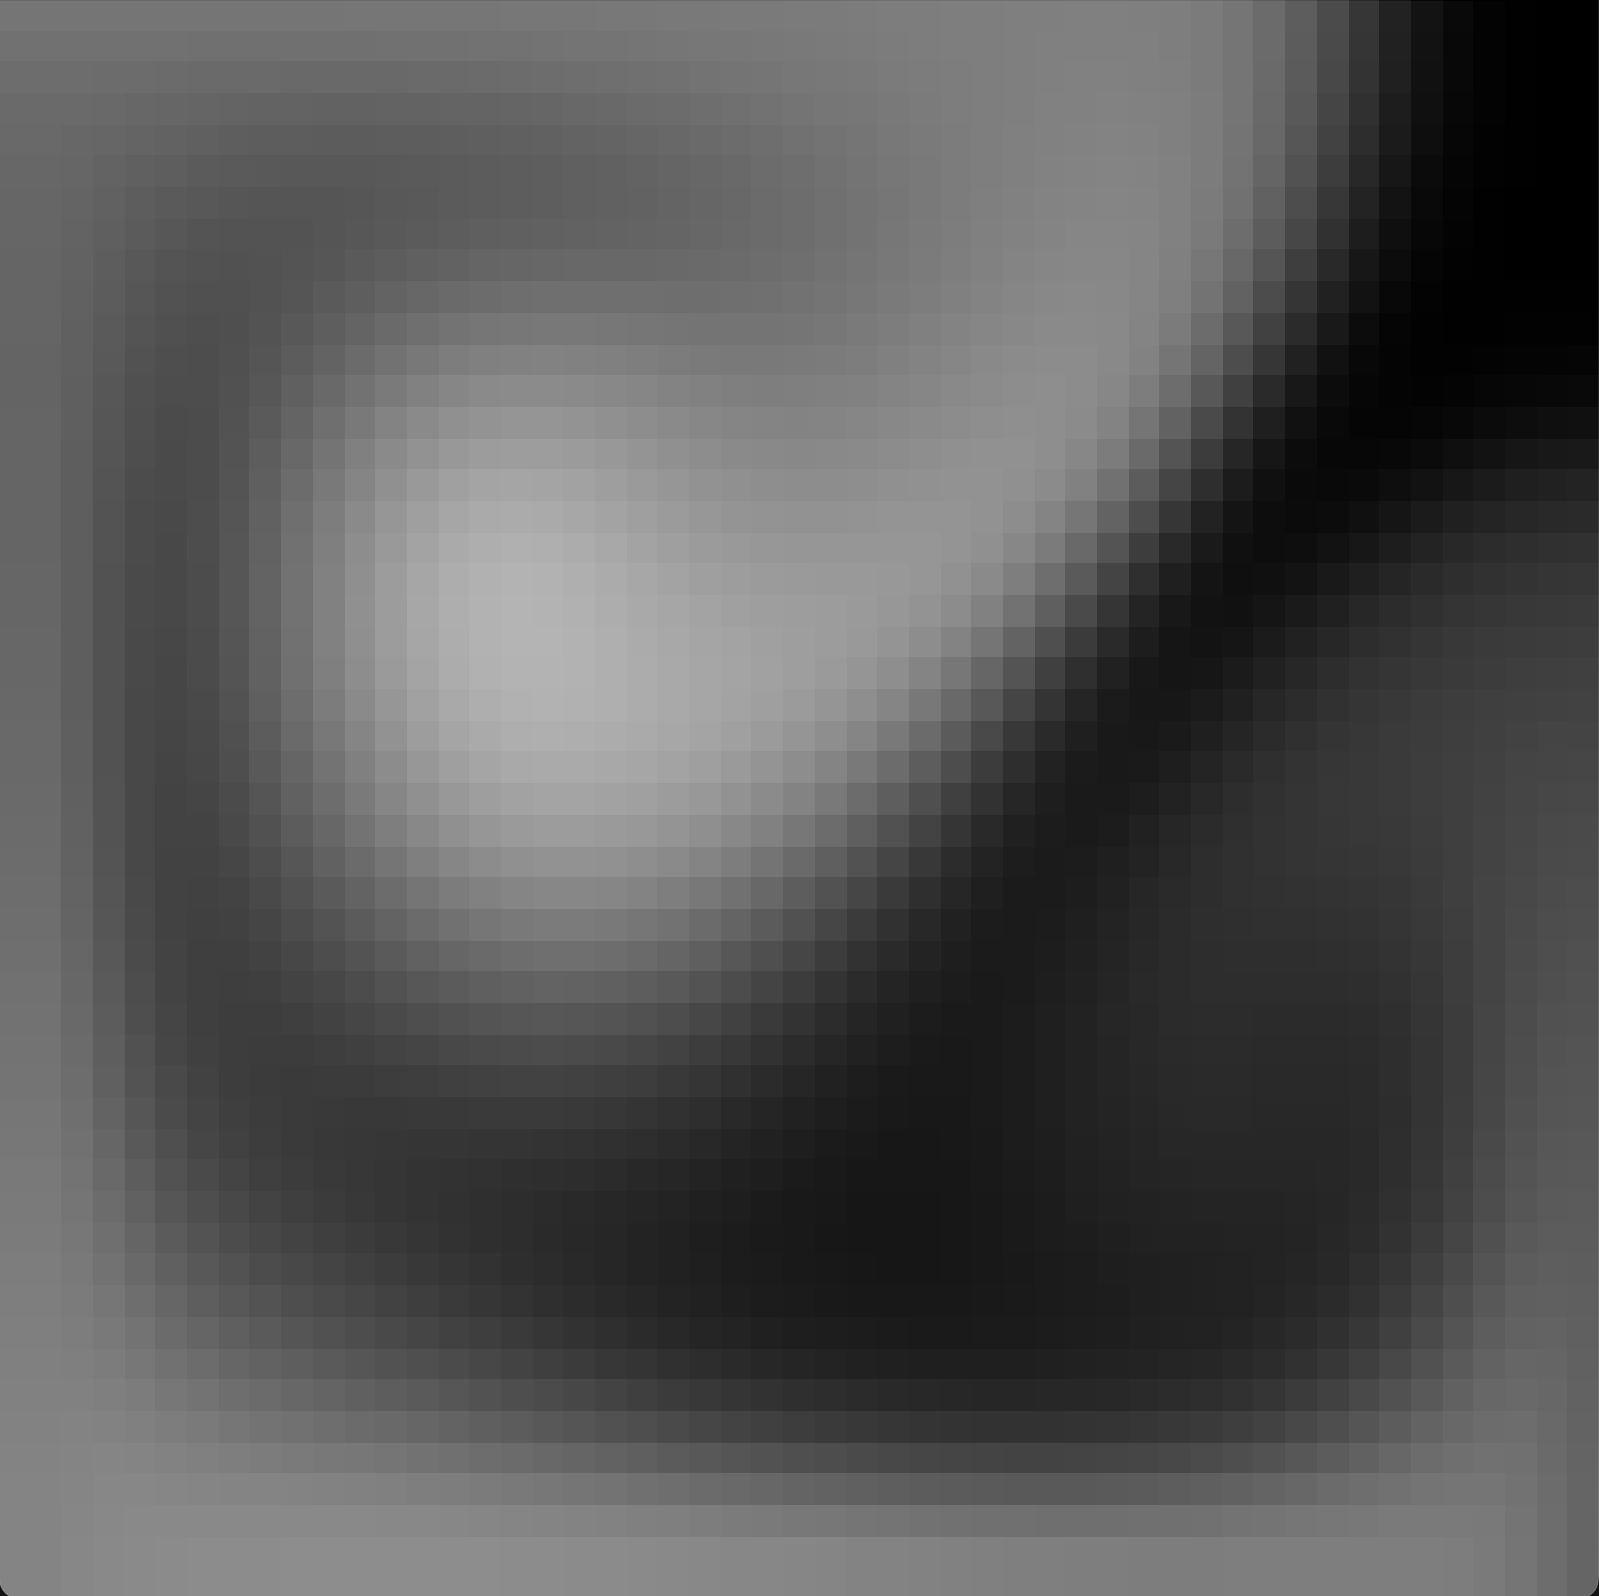
\includegraphics[width=\textwidth]{figures/grid50_3.png}
        \caption{third stage}
    \end{subfigure}
    \caption{Stages of Stable Fluids simulation 
    (a) shows the initial grid configuration
    (b)–(d) show different stages of the simulation}
    \label{fig:grid}
\end{figure*}

\subsection{PIC and PIC/FLIP}

We tested both the PIC and PIC/FLIP methods with the same number of particles. Figure~\ref{fig:pic_comparison} shows the final result of the simulation using each method.

The PIC method loses energy fast. Particles move less and quickly fall to the bottom.
The PIC/FLIP method keeps more energy. Particles move more and look more natural.

\begin{figure*}[h]
    \centering
    \begin{subfigure}[b]{0.4\textwidth}
        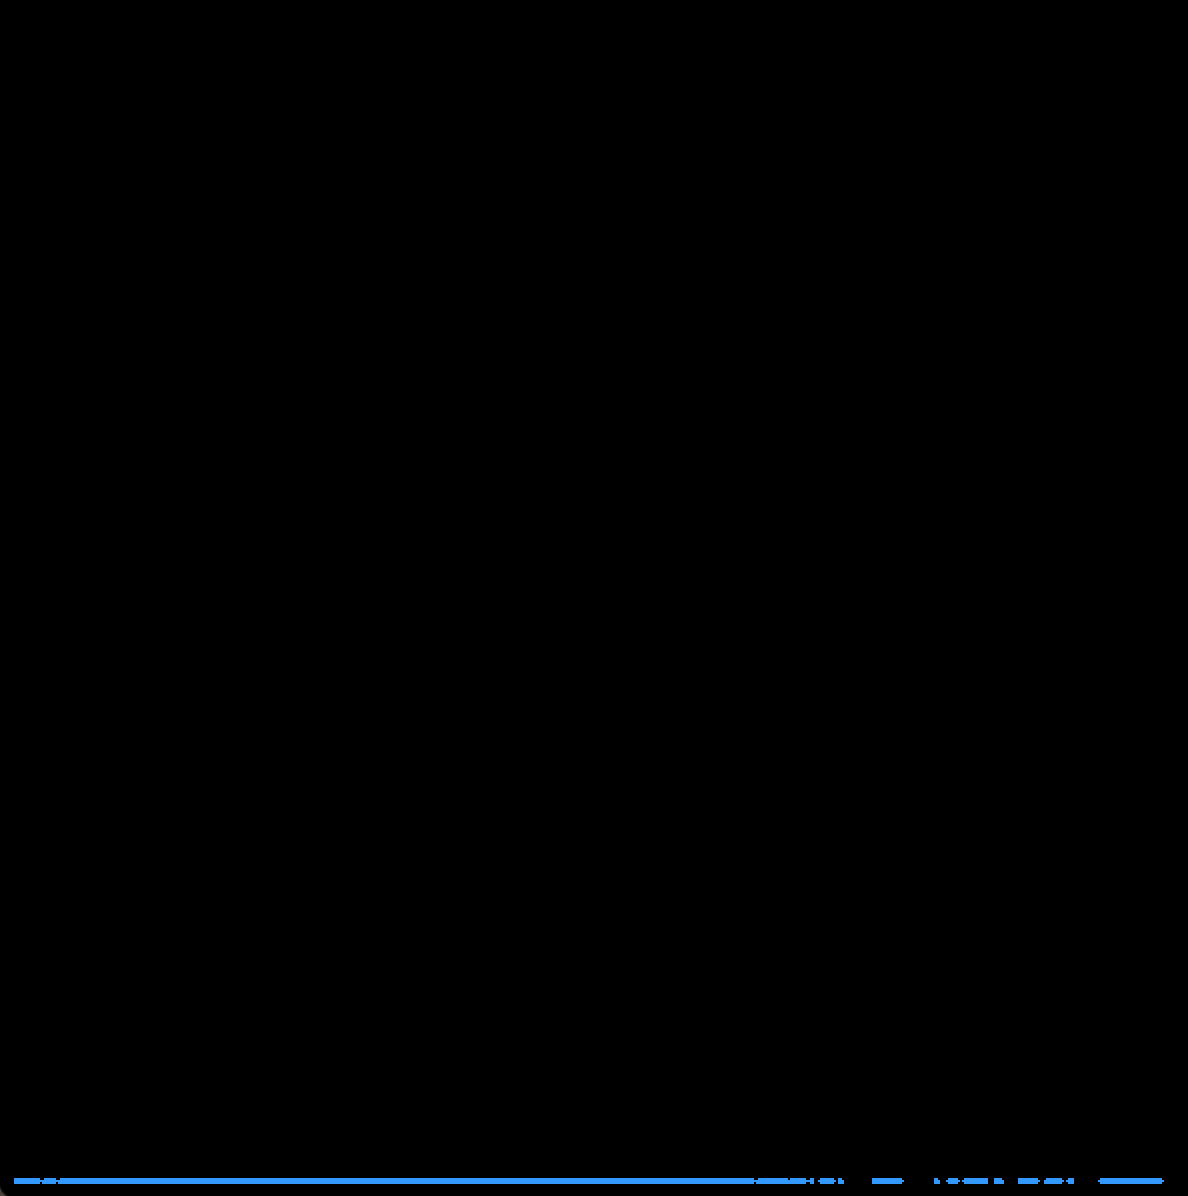
\includegraphics[width=\textwidth]{figures/pic_result.png}
        \caption{PIC result: motion is more damped.}
    \end{subfigure}
    \hspace{0.05\textwidth}
    \begin{subfigure}[b]{0.4\textwidth}
        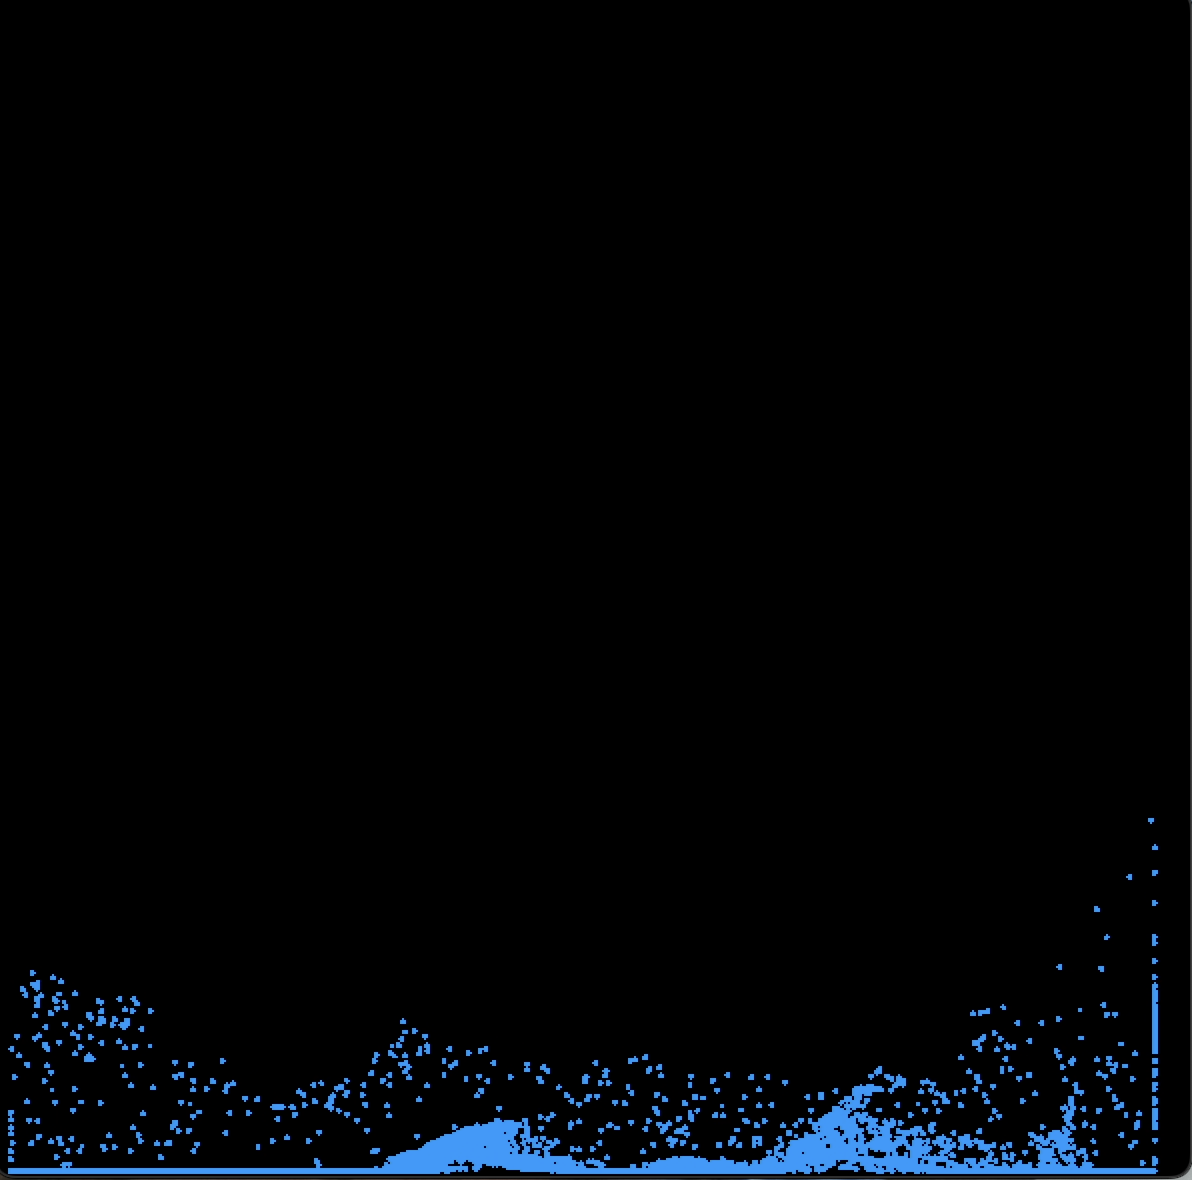
\includegraphics[width=\textwidth]{figures/pic_flip_result.png}
        \caption{PIC/FLIP result: motion is more dynamic.}
    \end{subfigure}
    \caption{Final particle positions using PIC and PIC/FLIP. Both start from the same initial state, but show different behavior due to how velocity is transferred.}
    \label{fig:pic_comparison}
\end{figure*}

\subsection{APIC}

We evaluated the performance of the APIC method with different particle counts. Figure~\ref{fig:apic_comparison} shows simulation snapshots at three resolutions—1000, 4000, and 8000 particles—demonstrating how the method handles fluid detail, stability, and distribution over time. Each subfigure compares the final state of the fluid, and highlights how increasing the number of particles leads to smoother, more detailed results.

\begin{figure*}[h]
    \centering
    \begin{subfigure}[b]{0.2\textwidth}
        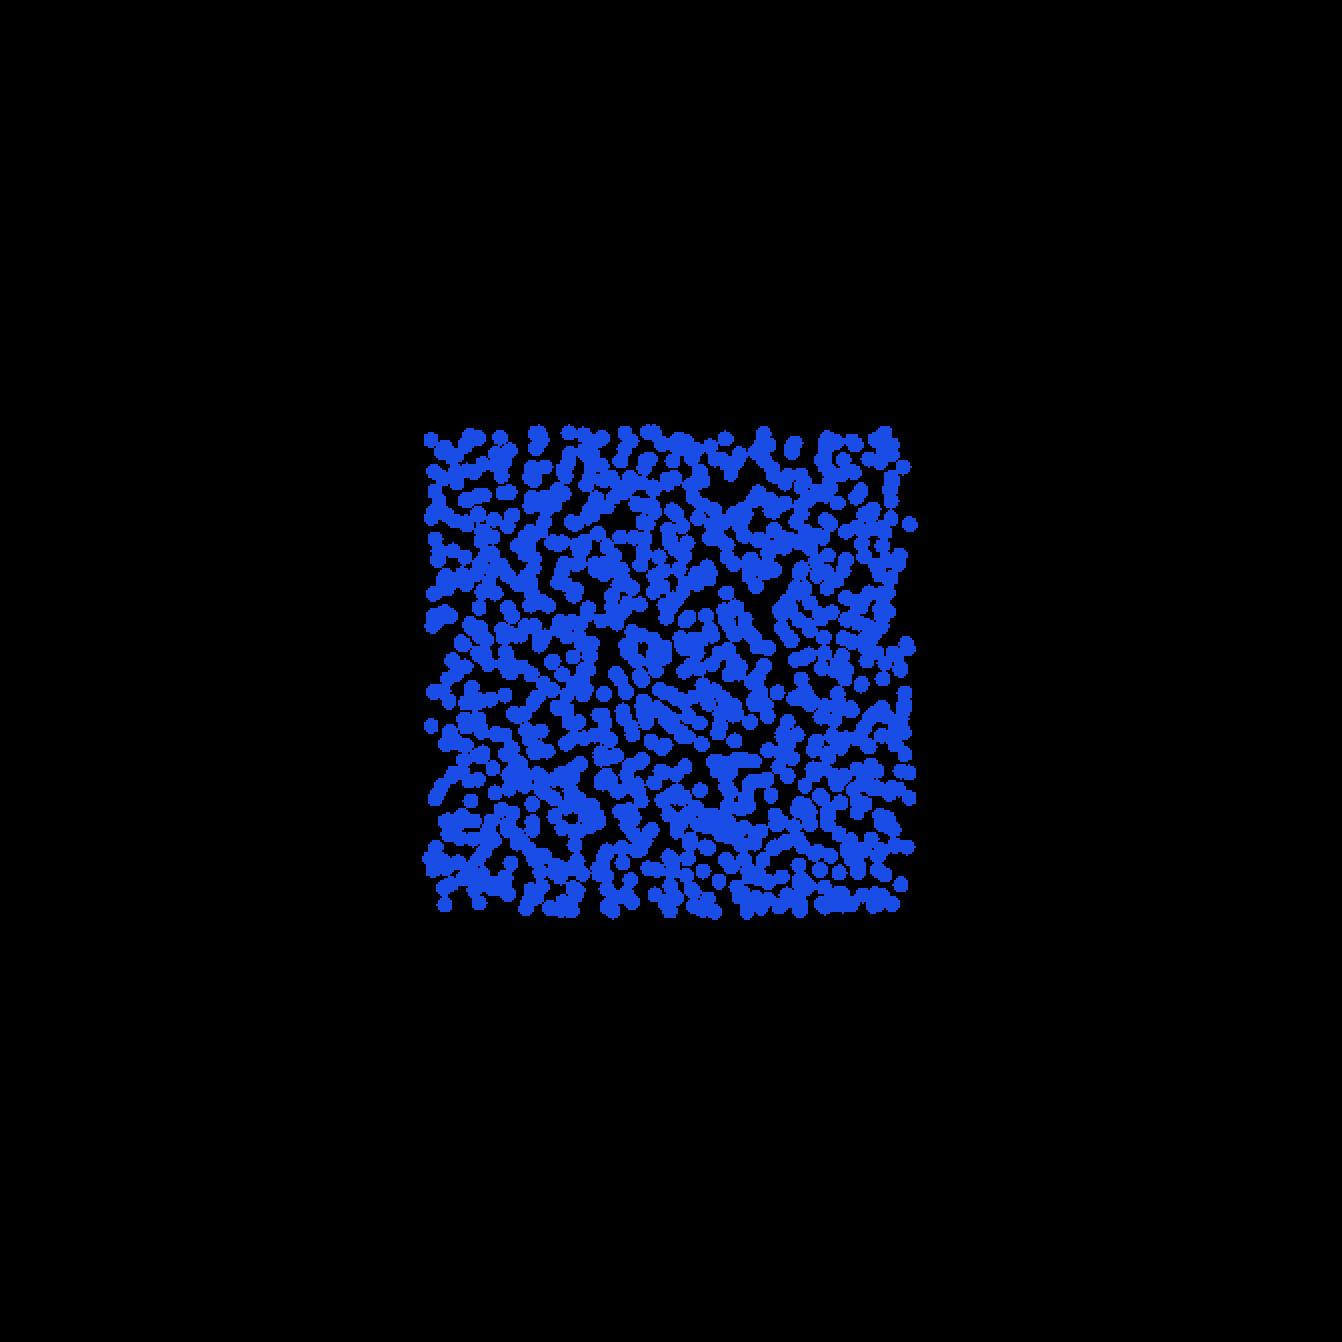
\includegraphics[width=\textwidth]{figures/apic1000_init.png}
        \caption{1000 initial particles}
    \end{subfigure}
    \hspace{1em}
    \begin{subfigure}[b]{0.2\textwidth}
        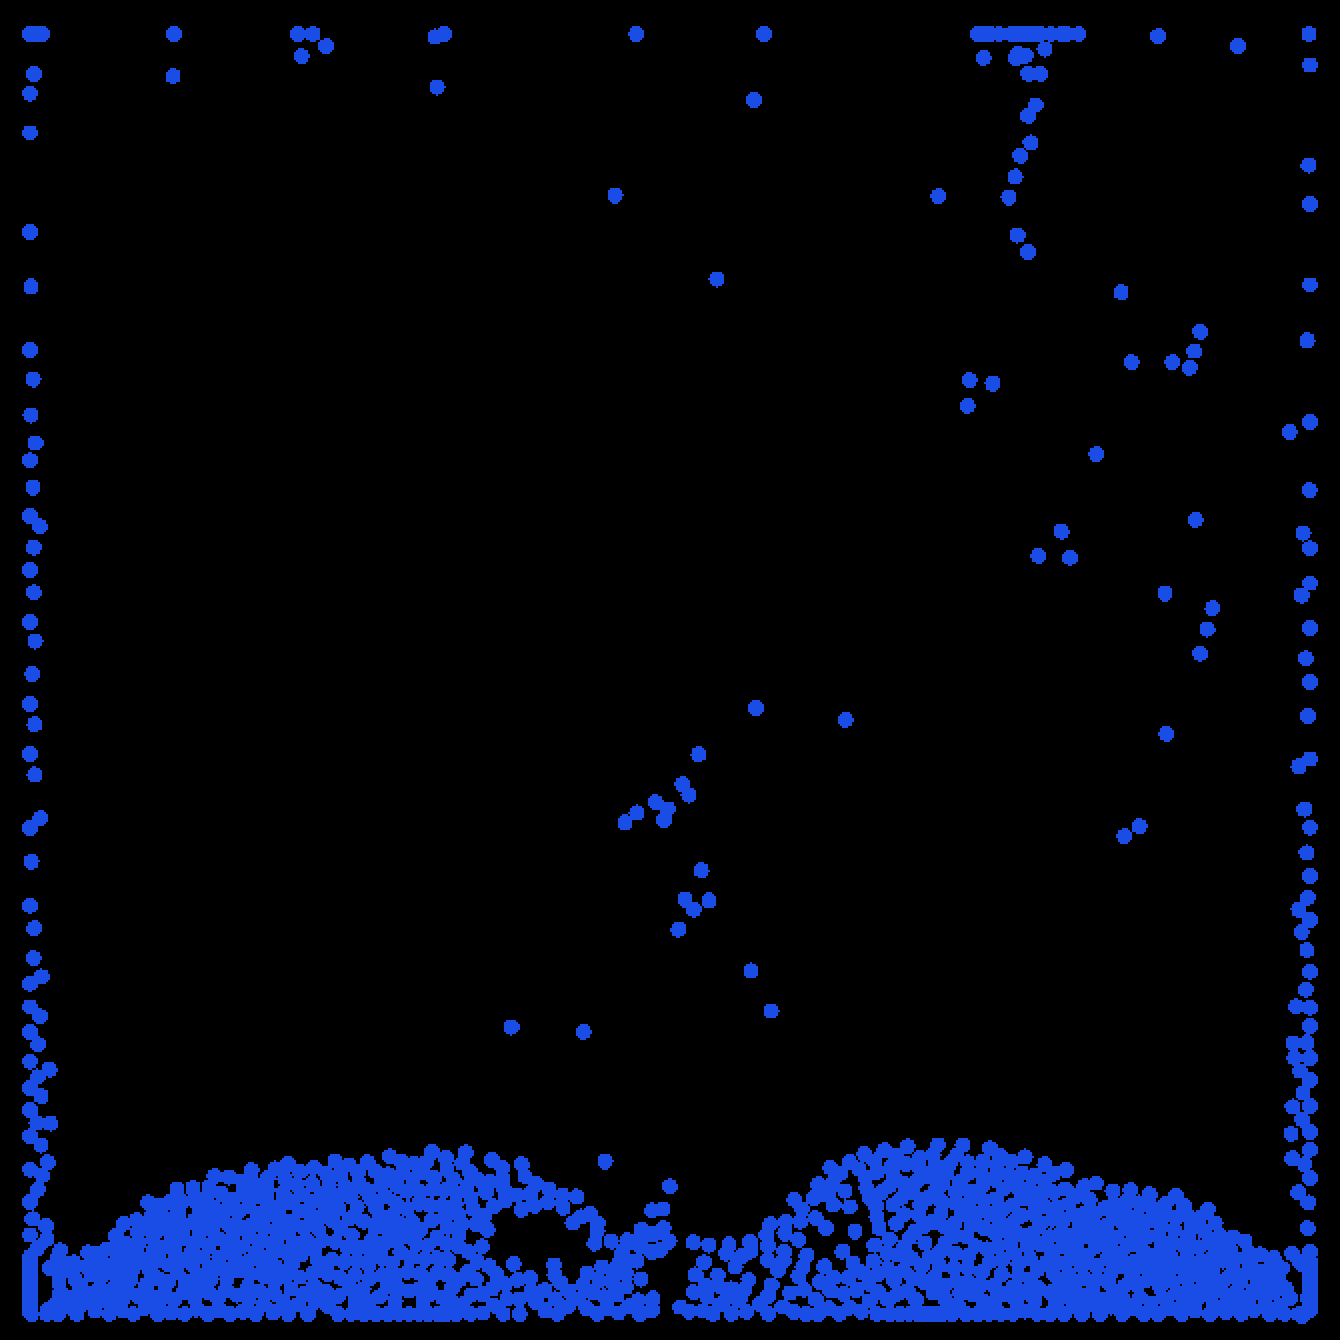
\includegraphics[width=\textwidth]{figures/apic1000.png}
        \caption{1000 particles}
    \end{subfigure}
    \hspace{1em}
    \begin{subfigure}[b]{0.2\textwidth}
        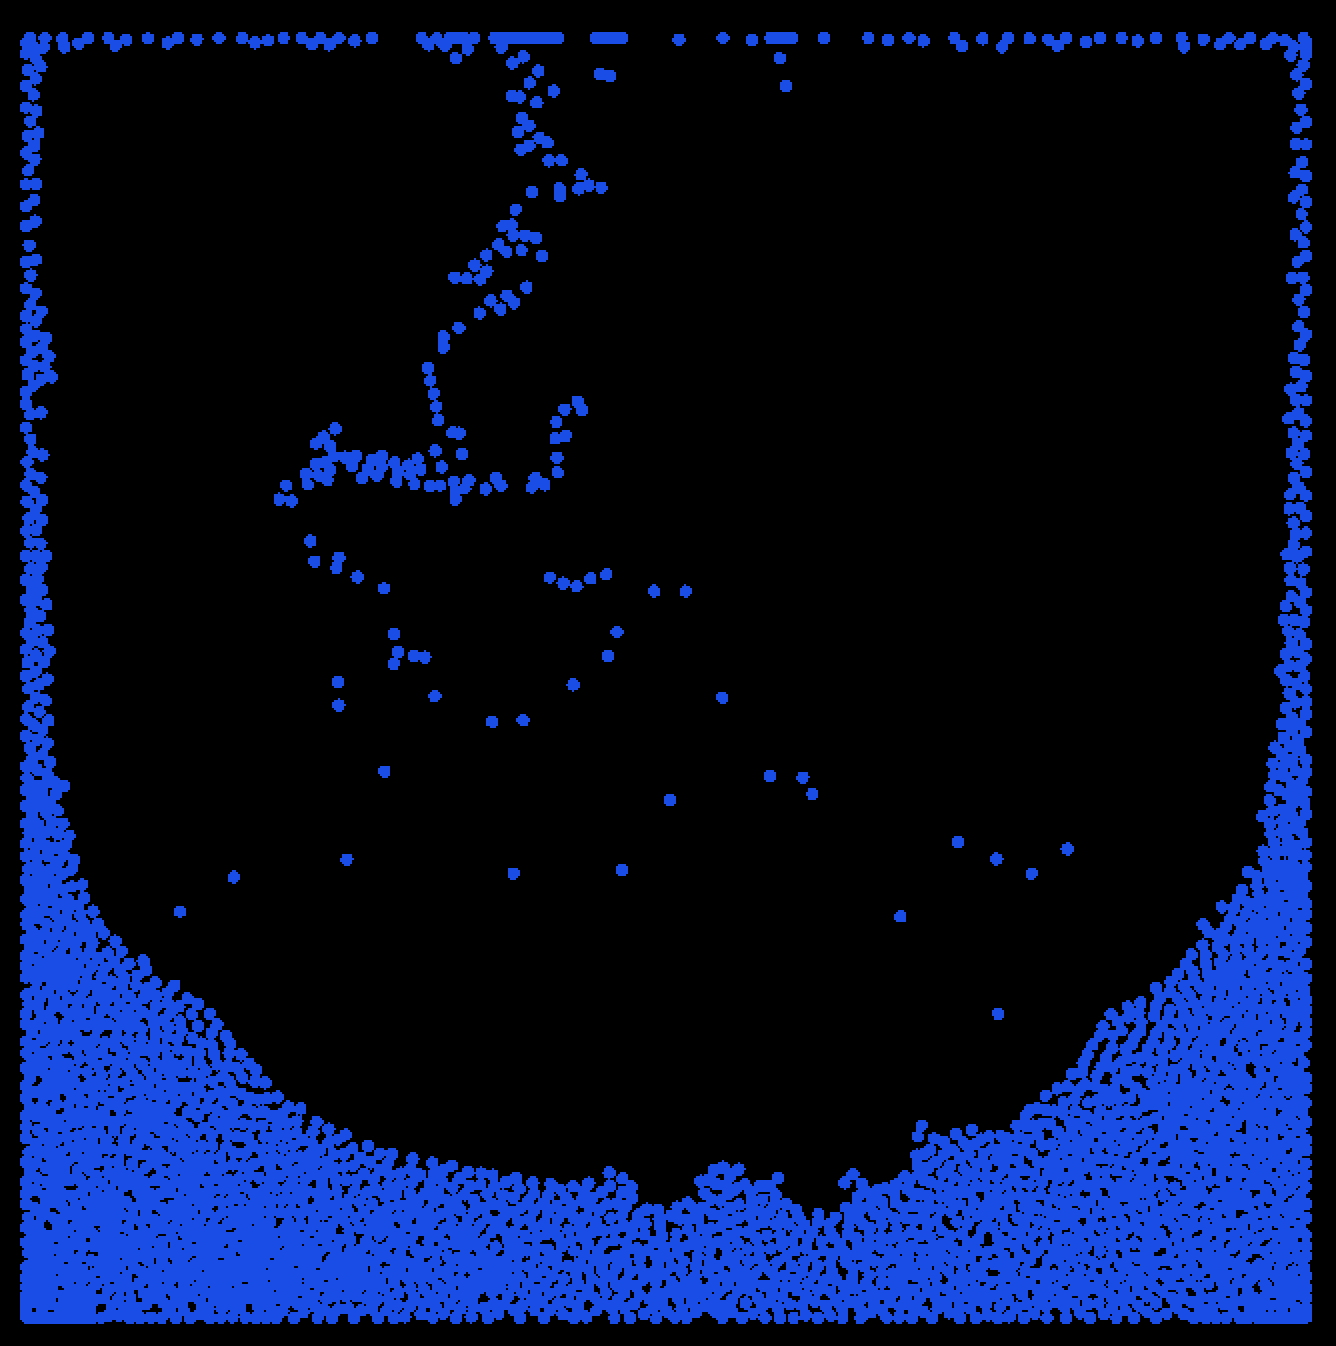
\includegraphics[width=\textwidth]{figures/apic4000.png}
        \caption{4000 particles}
    \end{subfigure}
    \hspace{1em}
    \begin{subfigure}[b]{0.2\textwidth}
        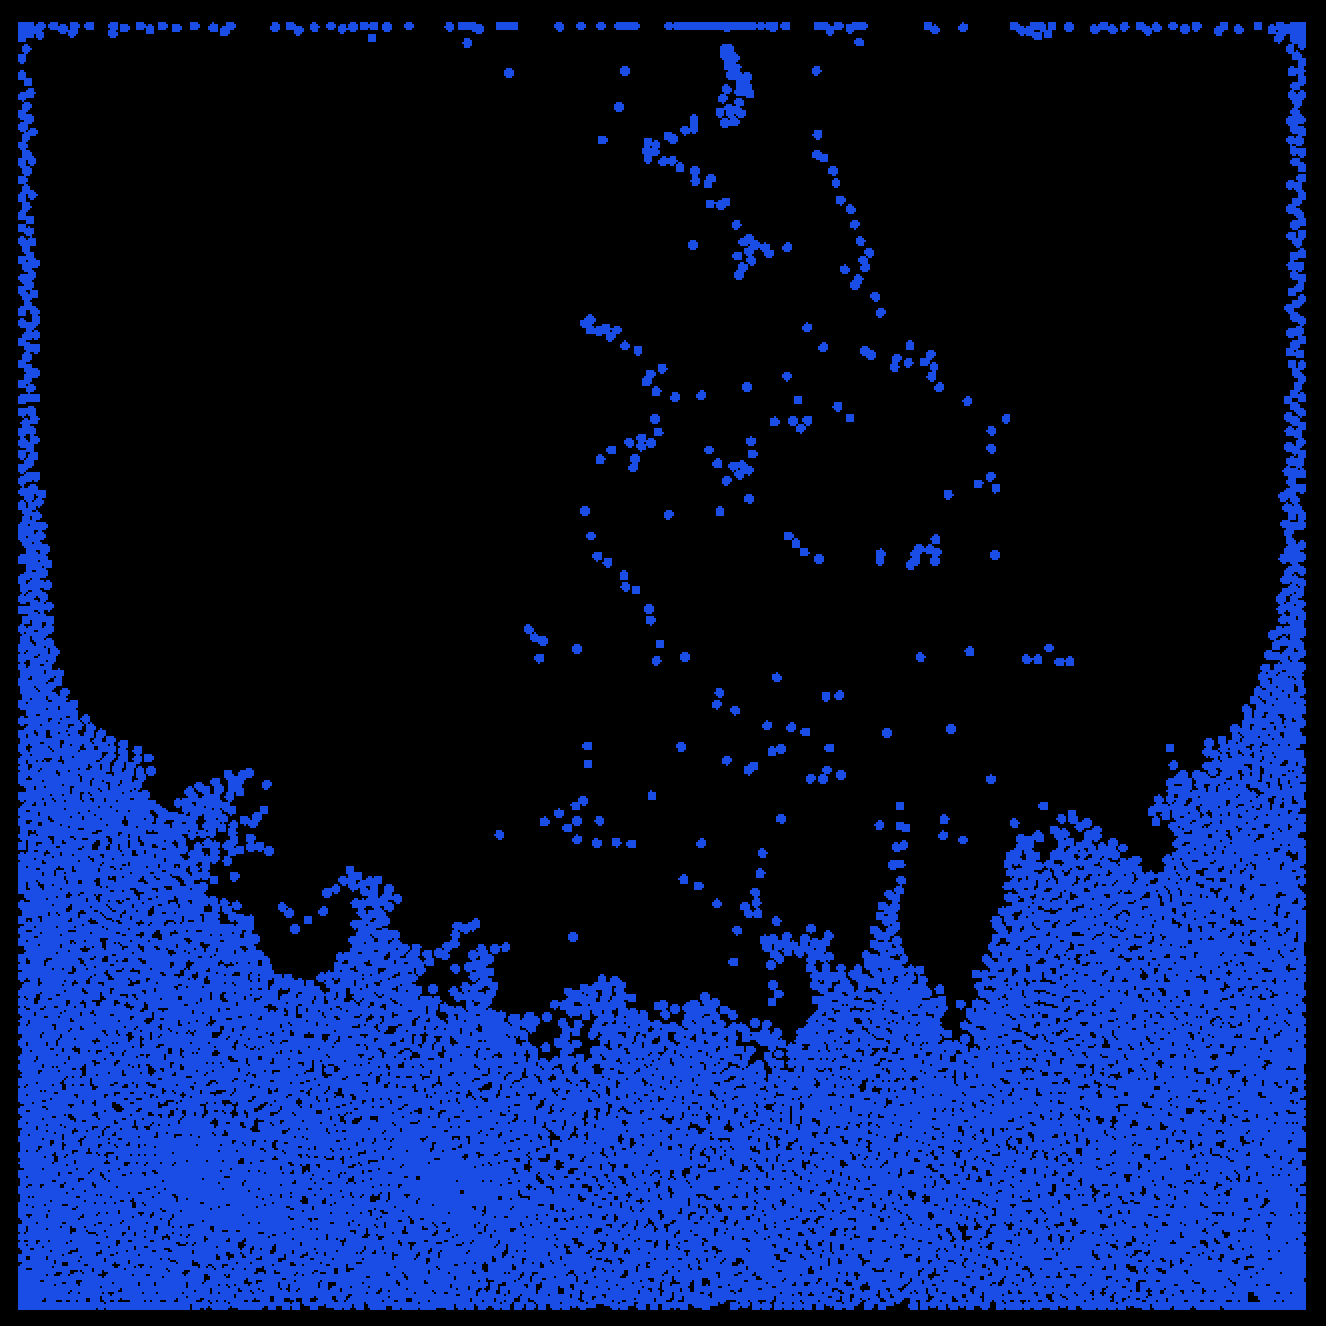
\includegraphics[width=\textwidth]{figures/apic8000.png}
        \caption{8000 particles}
    \end{subfigure}
    \caption{Comparison of APIC simulation results with increasing particle counts. 
    (a) shows the initial particle configuration, where all particles are placed in the center of the domain. 
    (b)–(d) show the simulation at the moment particles start to fall under gravity.}
    \label{fig:apic_comparison}
\end{figure*}